\documentclass[a4paper,12 pt]{article}
\usepackage[T2A]{fontenc}
\usepackage[utf8]{inputenc}
\usepackage[english, russian]{babel}
\usepackage{geometry}
\usepackage{float}
\usepackage{amsfonts}
\usepackage{array}
\newcolumntype{C}[1]{>{\centering\arraybackslash}p{#1}}
 \geometry{
 a4paper,
 top=25mm,
 }
\usepackage{amsmath, amsfonts, amssymb, amsthm, mathtools, indentfirst, float, wrapfig}
\usepackage{graphicx}
\begin{document}
    \begin{titlepage}
    \begin{center}
        \vspace{4cm}
        \huge {\textbf{Отчет о выполнении лабораторной работы 1.4.8 }}
        {} \\
        \vspace{1cm}
        \Large {\textbf{Измерение модуля Юнга}} \\
        \Large {\textbf{методом акустического резонанса}} \\
        \vspace{10cm}
        \begin{flushright}
        \begin{minipage}{.45\textwidth}
        \normalsize{\textbf{Студент:} Копытова Виктория Сергеевна}\\
        \textbf{Группа:} Б03-304\\
        \end{minipage}
        \end{flushright}   
    \end{center}
    \end{titlepage}
\newpage
 
\section{Аннотация}
\textbf{Цель работы:} исследовать явление акустического резонанса в тонком стержне; измерить скорость распространения продольных звуковых колебаний в тонких стержнях из различных материалов и различных размеров; измерить модули Юнга различных материалов.

\textbf{В работе используются:} генератор звуковых частот, частотомер, осциллограф, электромагнитные излучатель и приёмник колебаний, набор стержней из различных материалов.
	

\section{Теоретические сведения}

Основной характеристикой упругих свойств твёрдого тела является его
модуль Юнга $E$. Согласно закону Гука, если к элементу среды приложено
некоторое механическое напряжение $\sigma$, действующее вдоль некоторой
оси $x$ (напряжения по другим осям при этом отсутствуют), то в этом эле-
менте возникнет относительная деформация вдоль этой же оси
$\varepsilon = \Delta x/x_0$, определяемая соотношением
\begin{equation}
    \sigma = \varepsilon E
\end{equation}

Если с помощью кратковременного воздействия в некотором элементе
твёрдого тела создать малую деформацию, она будет далее распространяться в среде в форме волны, которую называют акустической или звуковой.
Cкорость $u$ распространения продольной акустической волны в простейшем случае длинного тонкого стержня определяется соотношением
\begin{equation}
    u = \sqrt{\frac{E}{\rho}},
\end{equation}
где $\rho$ - плотность среды, при условии, что длина волны гораздо больше радиуса стержня $\lambda \gg R$ и $\varepsilon \ll 1$.

\textbf{Стоячие волны}

В случае гармонического возбуждения колебаний с частотой $f$ продольная волна в тонком стержне может быть представлена в виде суперпозиции
двух бегущих навстречу гармонических волн:
\begin{equation}
    \xi (x,t) = A_1 \sin(\omega t -kx +\varphi_1) + A_2 \sin(\omega t -kx +\varphi_2),
\end{equation}
где $\omega = 2 \pi f$ -- циклическая частота, $k = 2 \pi / \lambda$ -- волновое число, $ \lambda$ -- длина волны.

Если концы стержня с координатами $x=0, x=L$ не закреплены, то напряжение в них
\begin{equation}
    \sigma(0) = 0 \rightarrow \frac{\partial \xi}{\partial x} =0, \quad \sigma(L) = 0 \rightarrow \frac{\partial \xi}{\partial x} =0
\end{equation}

Тогда соотношение (3) верно при любом $t$, если амплитуды и фазы падающей и отражённой волны одинаковы.
\begin{equation}
    \xi (x,t) = 2A \cos(kx) \sin(\omega t +\varphi).
\end{equation}

Колебания вида (5) называютя гармоническими стоячими волнами. 

Воспользуемя условием (4) и получим уравнение $\sin (kL) = 0$. Решения которого
\begin{equation}
    k_n L = \pi n, \quad n \in \mathbb{N},
\end{equation}
\begin{equation}
    \lambda_n = \frac{2L}{n}, \quad n \in \mathbb{N}.
\end{equation}

Таким образом, для возбуждения стоячей волны на длине стержня должно
укладываться целое число полуволн.

Допустимые значения частот
\begin{equation}
    f_n = \frac{u}{\lambda_n} = n \frac{u}{2L}, \quad n \in \mathbb{N}.
\end{equation}
называют собственными частотами колебаний стержня длиной $L$.
Именно при совпадении внешней частоты с одной из частот $f_n$ в стержне
возникает акустический резонанс.

\textbf{Экспериментальная установка}
\begin{figure}[H]
    \centering
    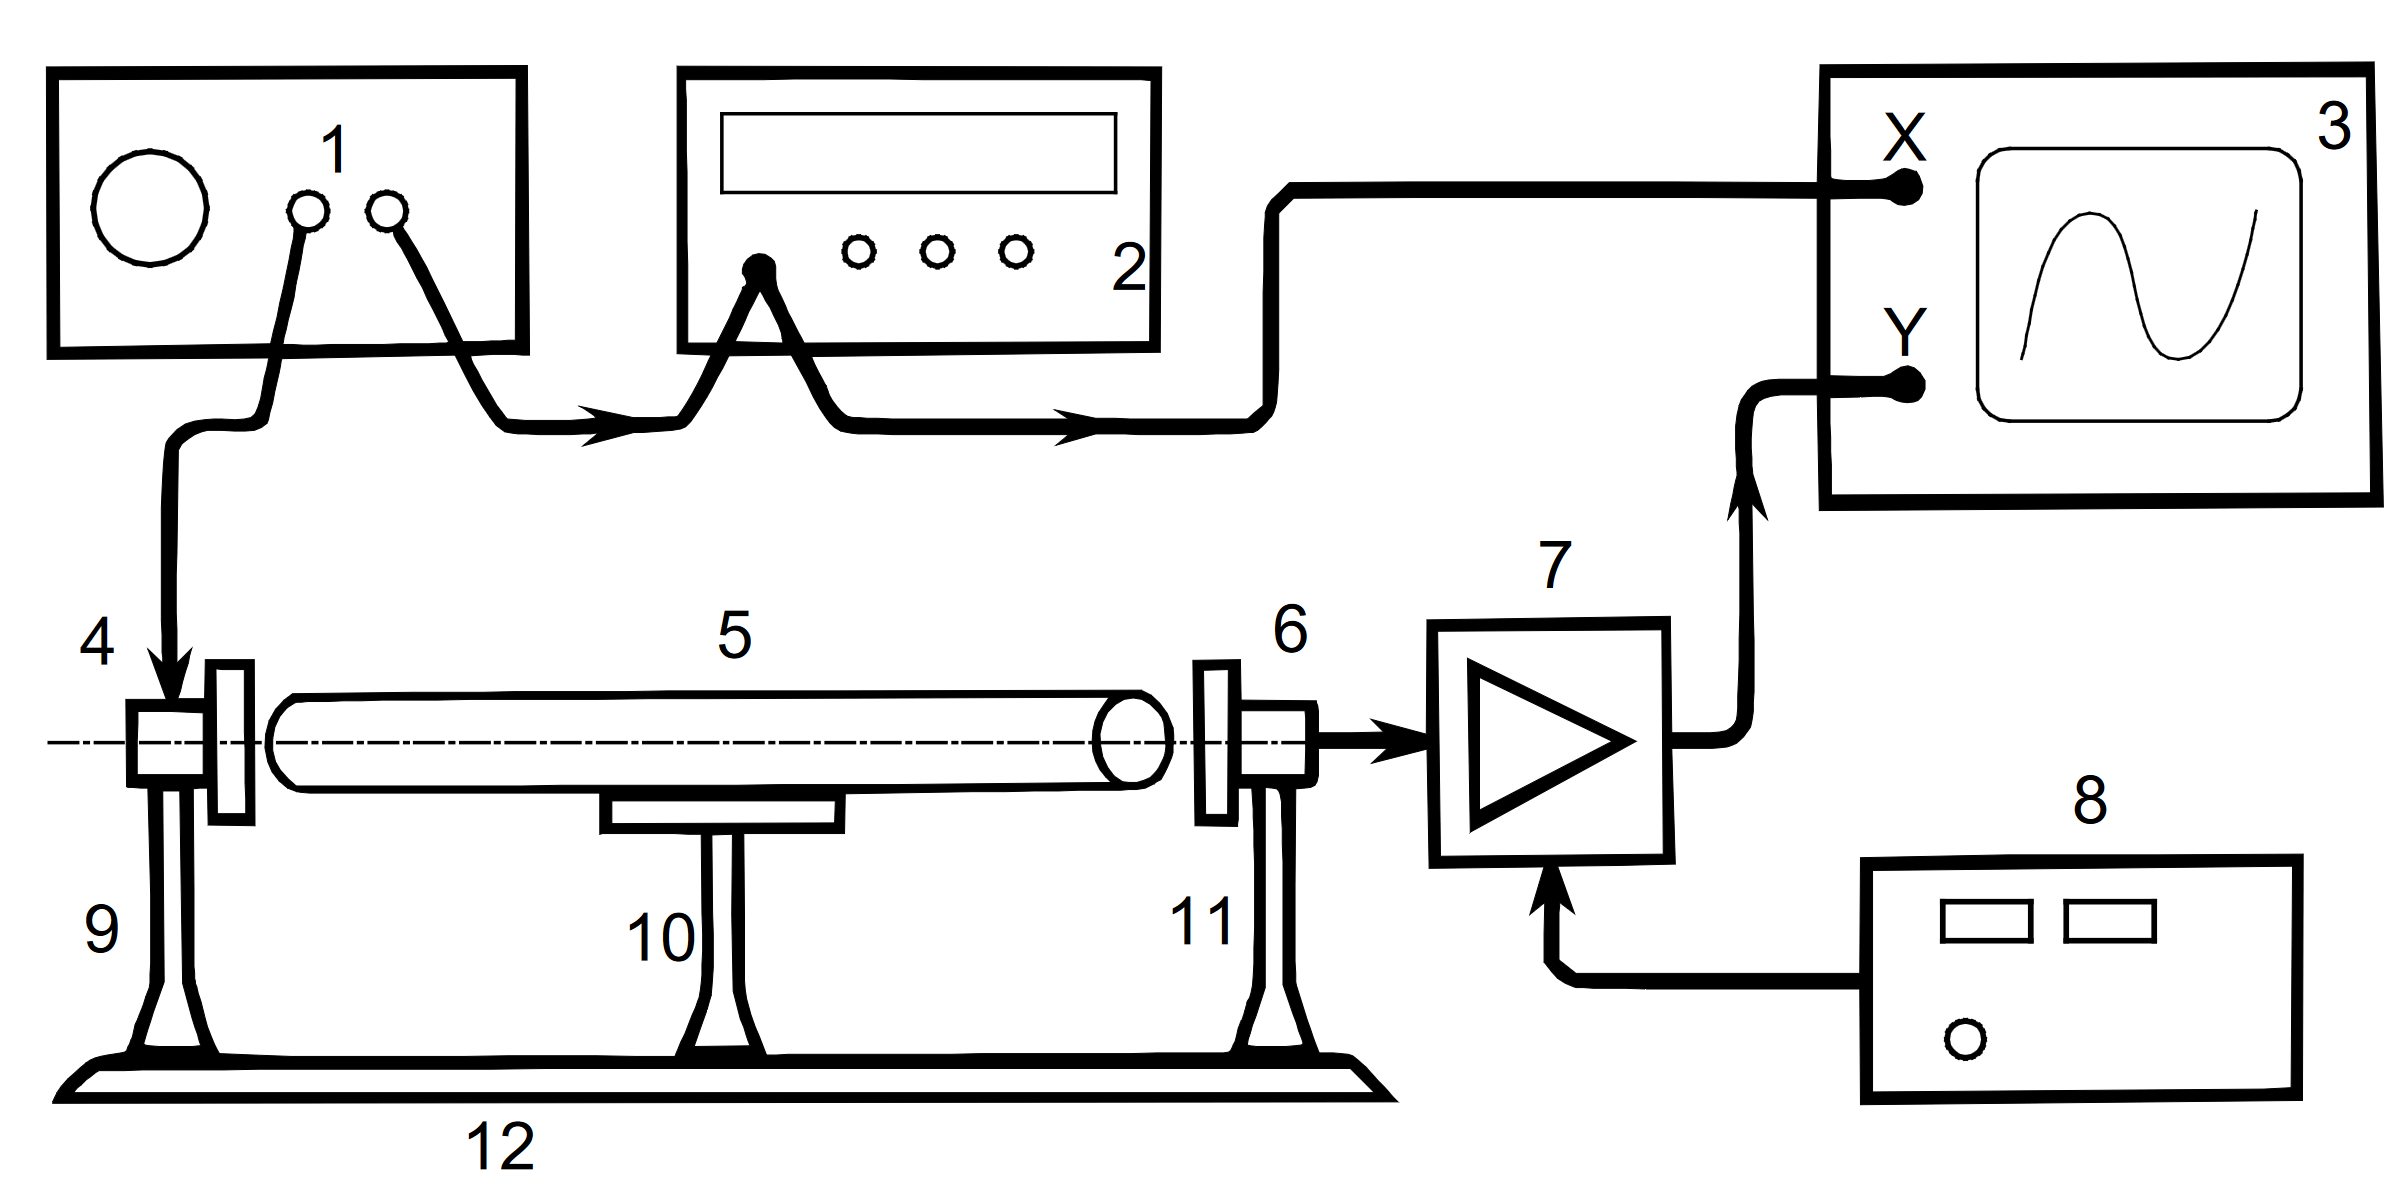
\includegraphics[scale = 0.3]{установка.png}
    \caption{Схема установки: 1 -- генератор звуковой частоты, 2 -- частотомер,
3 – осциллограф, 4 -- электромагнит-возбудитель, 5 -- образец, 6 -- электромагнит-приёмник, 7 -- усилитель звуковой частоты, 8 -- блок питания усилителя, 9, 11 -- стойки крепления электромагнитов, 10 -- стойка крепления образца, 12 -- направляющая}
\end{figure}

Схема экспериментальной установки приведена на рис. 3. Исследуемый стержень 5 размещается на стойке 10. Возбуждение и приём колебаний в стержне осуществляются электромагнитными преобразователями 4 и 6, расположенными рядом с торцами стержня. Крепления 9, 11 электромагнитов дают возможность егулировать их расположение по высоте, а также перемещать вправо-влево по столу 12.

Электромагнит 4 служит для возбуждения упругих механических продольных колебаний в стержне. На него с генератора звуковой частоты 1 подаётся сигнал синусоидальной формы: протекающий в катушке электромагнита ток создаёт ропорциональное ему магнитное поле, вызывающе епериодическое воздействие заданной частоты на торец стержня (к торцам стержней из немагнитных материалов прикреплены тонкие стальные шайбы). Рядом с другим торцом стержня находится аналогичный электро магнитный датчик 6, который служит для преобразования механических колебаний в электрические. 

Сигнал с выхода генератора поступает на частотомер 2 и на вход канала X осциллографа 3. ЭДС, возбуждаемая в регистрирующем электромагните 6, пропорциональная амплитуде колебаний торца стержня, усиливается усилителем 7 и подаётся на вход канала Y осциллографа.

\textbf{Методика измерений}

Для определения скорости $u$ в данной работе используется
метод акустического резонанса. Зная номер гармоники $n$ и соответствующую резонансную частоту $\nu_n$, на которой наблюдается усиление амплитуды колебаний,
можно вычислить скорость распространения продольных волн в стержне:
\begin{equation}
    u = 2L \frac{f_n}{n}.
\end{equation}



\section{Ход работы}

\begin{enumerate}
    \item Поместим стержень длиной $L = 600 \pm 0.5$ мм на подставку 10 и разместим электромагниты напротив торцов стрежня, не допуская их соприкосновения.
    \item Оценим частоту первого резонанса по формуле $f_1 = u/2L$, воспользовавшись табличным значение скорости и медленно меняя частоту звукового генератора вблизи расчётной найдём первый резонанс.
    \item Найдём резонансы на следующих гармониках. Результаты занесём в таблицу 1.

\begin{table}[H]
    \centering
    \begin{tabular}{|C{1 cm}|C{3 cm}|C{3 cm}|C{3 cm}|}
        \hline
        n & $f_n$, кГц, медь & $f_n$, кГц, алюминий & $f_n$, кГц, сталь \\
        \hline
                1 & 3.160 & 4.261 & 4.125 \\
        \hline
                2 & 6.300 & 8.540 & 8.275 \\
        \hline
                3 & 9.486 & 12.78 & 12.38 \\
        \hline
                4 & 12.66 & 17.04 & 16.51 \\
        \hline
                5 & 15.81 & 21.30 & 20.63 \\
        \hline
                6 & 18.98 & 25.55 & 24.75 \\
        \hline
                7 & 22.12 & 29.79 & 28.86 \\
        \hline
                8 & 25.27 & 34.03 & 32.99 \\
        \hline
                9 & 28.51 & 38.26 & 37.08 \\
        \hline       
    \end{tabular}
    \caption{Резонансные частоты}
\end{table}
\begin{figure}[H]
    \centering
    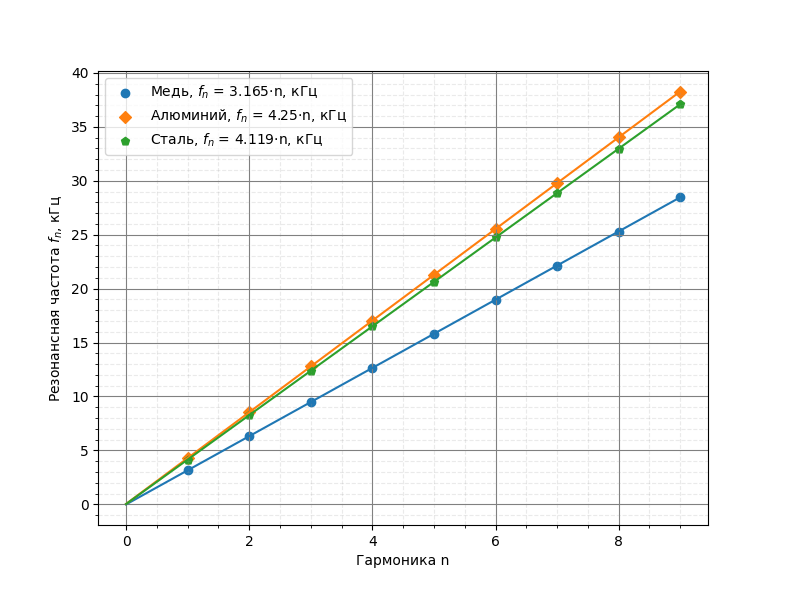
\includegraphics[scale=0.8]{резонанс.png}
    \caption{Зависимость резоннансной частоты от гармоники}
\end{figure}

Мы видим, что зависимость линейна и проходит через начало координат.
\item Определим плотности исследуемых материалов.

Измерим массу и размеры нескольких разных образцов каждого материала и усредним рассичтанные плотности. Получим
\begin{table}[H]
    \centering
    \begin{tabular}{|c|c|c|}
        \hline
        Материал & Плотность $\rho$, кг/$\text{м}^3$ & $\sigma_{\rho}$, кг/$\text{м}^3$ \\
        \hline
        Медь & 8.765 & 0.02 \\
        \hline
        Алюминий & 2.784 & 0.01 \\
        \hline
        Сталь & 7.842 & 0.02 \\
        \hline
    \end{tabular}
    \caption{Плотности материалов}
\end{table}
\item По коэффициенту наклона прямой определим скорость звука $u$ и модуль Юнга $E$.
\begin{displaymath}
    u = 2L \frac{f_n}{n}, \quad E = u^2 \rho
\end{displaymath}
\begin{table}[H]
    \centering
    \begin{tabular}{|C{2 cm}|C{2.5 cm}|C{1 cm}|C{2.5 cm}|C{1 cm}|C{1 cm}|}
        \hline
        Материал & Скорость звука $u$, км/с & $\sigma_u$, км/с & Модуль Юнга $E$, ГПа & $\sigma_E$, ГПа & $E_{\text{табл}}$, ГПа\\
        \hline
        Медь & 3.798 & 0.02 & 124.4 & 0.97 & 110-129\\
        \hline
        Алюминий & 5.100 & 0.02 & 72.41 & 0.48 & 68-74 \\
        \hline
        Сталь & 4.943 & 0.02 & 191.6 & 1.2 & 190-210  \\
        \hline
    \end{tabular}
    \caption{Cкорость звука и модуль Юнга}
\end{table}

\item Окончательные результаты
\begin{displaymath}
    E_{\text{меди}} = (124.4 \pm 0.97) \quad \text{ГПа}
\end{displaymath}

\begin{displaymath}
    E_{\text{алюминия}} = (72.41 \pm 0.48) \quad \text{ГПа}
\end{displaymath}

\begin{displaymath}
    E_{\text{стали}} = (191.6 \pm 1.2) \quad \text{ГПа}
\end{displaymath}


\end{enumerate}


\section{Вывод}

В ходе работы были получены значения модулей Юнга для меди, алюминия и стали, лежащие в пределах табличных значения для сплавов. Погрешность вычисления составила около 1\%. Основной вклад в пошрешность вносит погрешность измерения плотности материала. Также зависимость резонансной частоты не проходит точно через начало координат, поэтому погрешность полученного коэффициента $f_n/n$ достаточно велика. 
    

\end{document}


